% !TEX root = ../dissertation.tex

\chapter{Background}
\label{chapter:background}

\section{The basics of General Game Playing}

General Game Playing is a project of the Stanford Logic Group of Stanford University, California, which aims to create a platform for \gls{GGP}.
Since 2005, there have been annual \gls{GGP} competitions at the AAAI Conference.

A \gls{GGP} match consists of 3 major components:
\begin{itemize}
\item Game Description: The game rules, in \gls{GDL}.

\item Game Manager: This system acts as a referee and manages communication with the players and other systems like graphics for the spectators. \textit{State Data} is usually part of the Game Manager.

\item Players: Players are the most interesting component of a \gls{GGP} game, they need.

\end{itemize}

\begin{figure}[h]
	\centering
    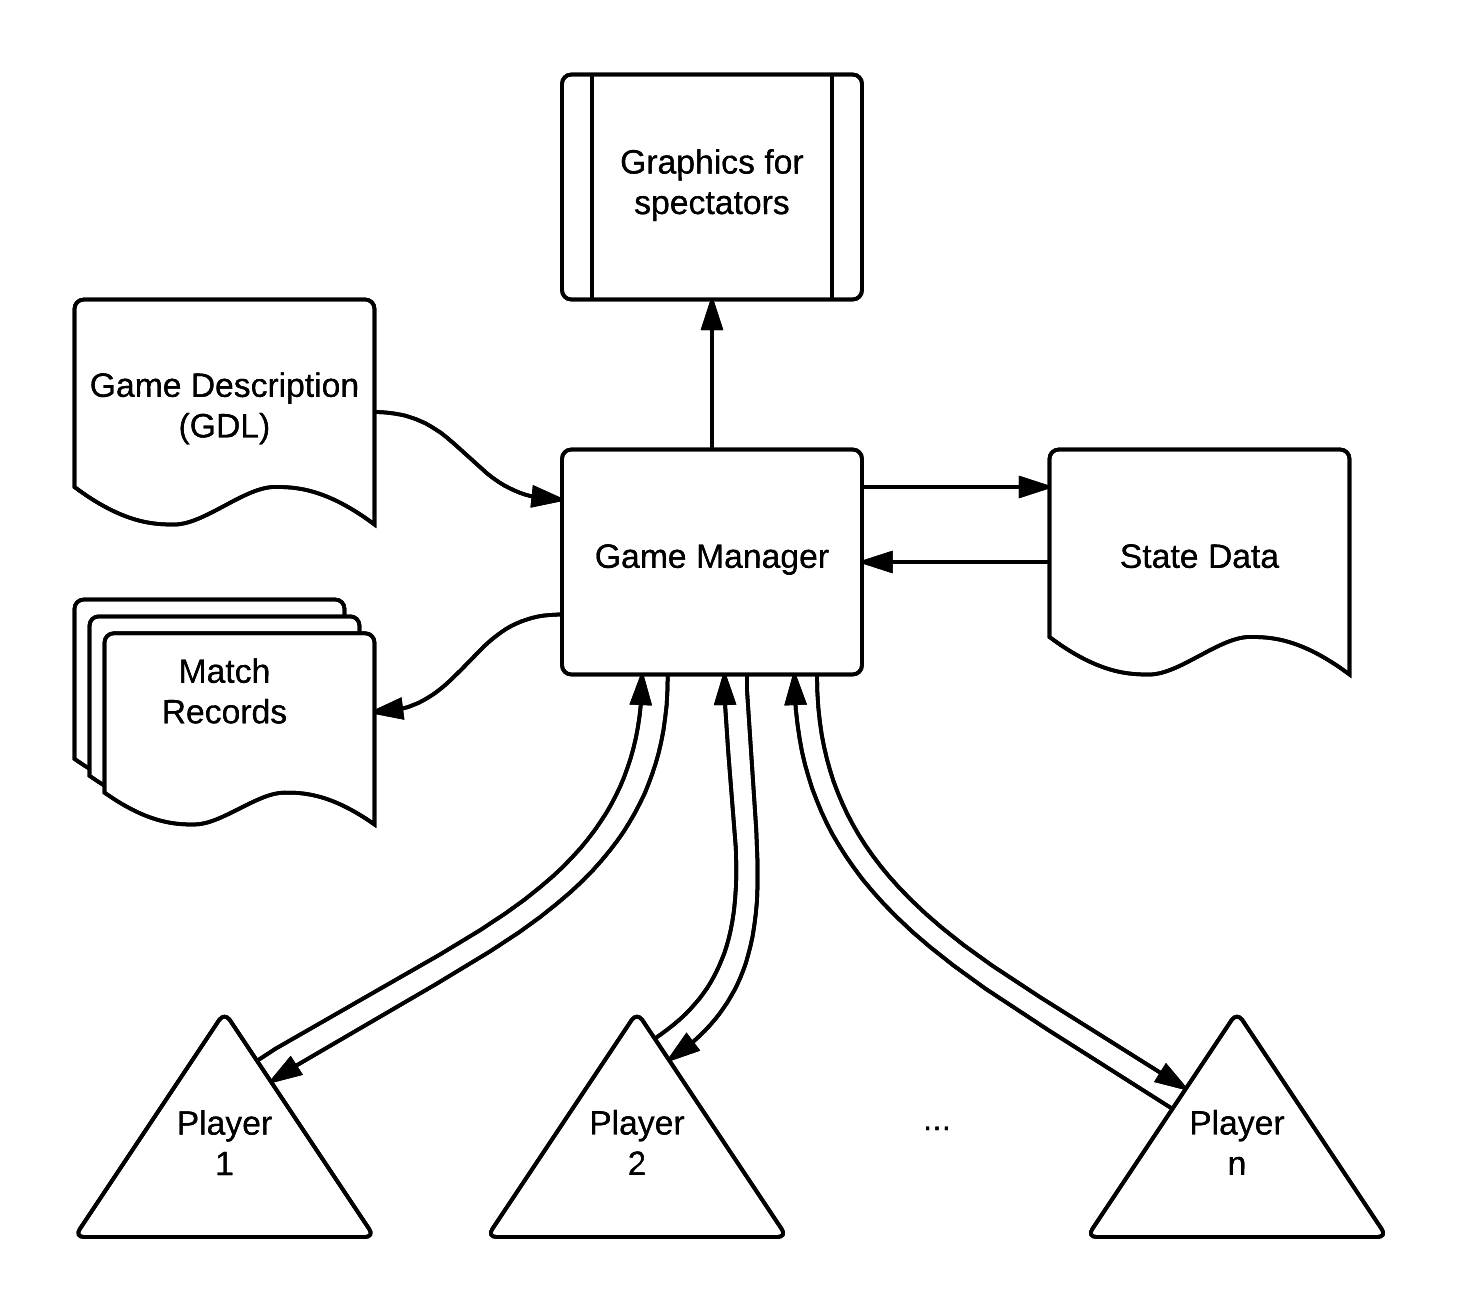
\includegraphics[scale=0.75]{images/GGPgamesetup.png}
    \caption{Match Components}
    \label{fig:match components}
\end{figure}

At the beginning of a match, the Game Manager sends all Players a match identifier, the game description, the role of each player and the time limits (for preparation (\textit{startclock}) and for each round (\textit{playclock})).

The match commences, after all players respond, with the Game Manager requesting a move from all players. Each round ends when all players send their moves or the time limit runs out (a random legal move is chosen for players that don't respond in time), after which the Game Manager will send each player another request along with all moves taken in the previous round.


\subsection{Game Description Language}
The \gls{GDL} is the standard way of describing games in the \gls{GGP} community.
\gls{GGP} players interpret the language using something called a \textit{Reasoner}. Choosing a good way of interpreting the game rules is one of the keys to performance and so many players develop their own custom \textit{reasoners}.

It can describe any finite deterministic move-based strategy game with an arbitrary number of players (most board games). GDL-II is an extension that has been made to allow for probabilistic games and incomplete information, like most card games.

Both GDL and GDL-II are variants of Datalog (query and rule language similar to prolog) and use first order logic.
Since GDL is a very conceptual description of the rules their interpretation is very computationally expensive. Choosing a good way of doing this interpretation (components that do this are called reasoners) is therefore very important to player performance, even in the recent years.

An example of tic tac toe described in GDL with some syntax explanation can be seen in \ref{appendix:gdl_example}

\subsection{Game Manager}
The purpose of the Game Manager is to be a single source of truth about what's happening in a match, and verify all moves taken by players. It must be able to interpret \gls{GDL}, to verify these moves

Players communicate their moves to the Game Manager (via HTTP), who checks the validity of the moves. A random legal move is chosen if a player chooses an illegal move or doesn't respond in time.

It should also provide a way of archiving the match history (all game states and moves taken) and other useful features like an interface for spectating.

\subsection{Game Player}
Game Players are systems that can interpret a \gls{GDL} game description, communicate with the Game Manager and devise strategies to maximize their result in a certain game.
Their aim is to be as general as possible while also having reasonably good performance in any game, which is a surprisingly difficult feat. Suffice it to say, sophisticated AI techniques like heuristics are very hard to successfully apply in a general, domain independent, way.

\section{Markov Decision Problem}
The \gls{MDP} provides a way of mathematically modeling decision making and can help to formalize the task of GGP Players.
In short, a Markov Decision Process is composed of 5 components:

\begin{itemize}
\item States - $S$ : The set of all possible states of the problem.

\item Actions - $A(s)$ : The set of possible actions in state $s$.

\item Model - $T(s, a, s') \sim Pr(s' | s, a)$ : The laws of the universe in which the problem is contained. In other words, what is the outcome (state $s'$) of taking an action $a$ in state $s$. The model can be deterministic or stochastic ($Pr(s' | s, a)$), where multiple outcomes are possible.

\item Reward - $R(s, a, s')$ : What is the reward of taking action $a$ in state $s$ and transitioning to state $s'$.

\item Discount Factor - $\gamma$ : Reduces the importance of distant rewards. It's important in the common case of a stochastic problem, since distant rewards may become unreachable due to external influence.
\end{itemize}

A policy, $\pi$, defines what action $\pi(s)$ the agent will take when in state $s$. Policies are solutions to \gls{MDP}'s.

In the domain of General Game Playing each different match has it's own \gls{MDP}, since the Model is defined not only by the game rules but also by the behavior of other players. Rewards and discount factors are also not solely dependent on the game rules (is it always a good move to take a Knight in chess?).
Most GGP matches have, therefore, unknown rewards and probabilities from the point of view of the player, making them \textit{reinforcement learning} problems. In these problems it is useful to define the function $Q(s,a)$, given by \ref{Q(s,a)}, and is an assessment of the quality of taking action $a$ in state $s$.

\begin{center}
\begin{equation} \label{Q(s,a)}
Q(s,a) = \sum_{s'} Pr(s' | s, a)(R(s, a, s') + \gamma V(s'))
\end{equation}
\end{center}

$V(s')$ is the value of being in state $s'$, the discounted sum of the expected rewards to be earned (on average) by following the policy from state $s'$ on-wards. There are several ways to implement this calculation.

If all the probabilities and rewards are known the policy can be solved recursively according to \ref{pi(s)} and \ref{V(s)}.

\begin{center}
\begin{equation} \label{pi(s)}
\pi(s) \equiv arg max_{a}\left \{ \sum_{s'} Pr(s' | s, a)(R(s, a, s') + \gamma V(s'))\right \}
\end{equation}
\end{center}

\begin{center}
\begin{equation} \label{V(s)}
V(s) \equiv \sum_{s'} Pr(s' | s, \pi(s))(R(s, \pi(s), s') + \gamma V(s'))
\end{equation}
\end{center}

\section{Basics of a GDL player}

A simplified example of a GGP Player architecture can be seen in figure \ref{fig:player architecture}. As seen in the figure, the player must have some form of these components:

\begin{itemize}
\item HTTP Server: Interfaces with the Game Master

\item \gls{GDL} Interpreter (also known as \textit{Reasoner}): Analyses the game rules, in some cases changing their representation into a more efficient data structure

\item Game State: Holds any relevant information about the game, like the current state or past moves by opponents (to maybe model their strategy)

\item Game Planner: Attempts to choose the best action for the current state of the game. If it uses simulations as part of its operation (very common) it may interface with the \textit{reasoner} to discover what actions are available in each of the simulated states.
\end{itemize}

\begin{figure}[h]
	\centering
    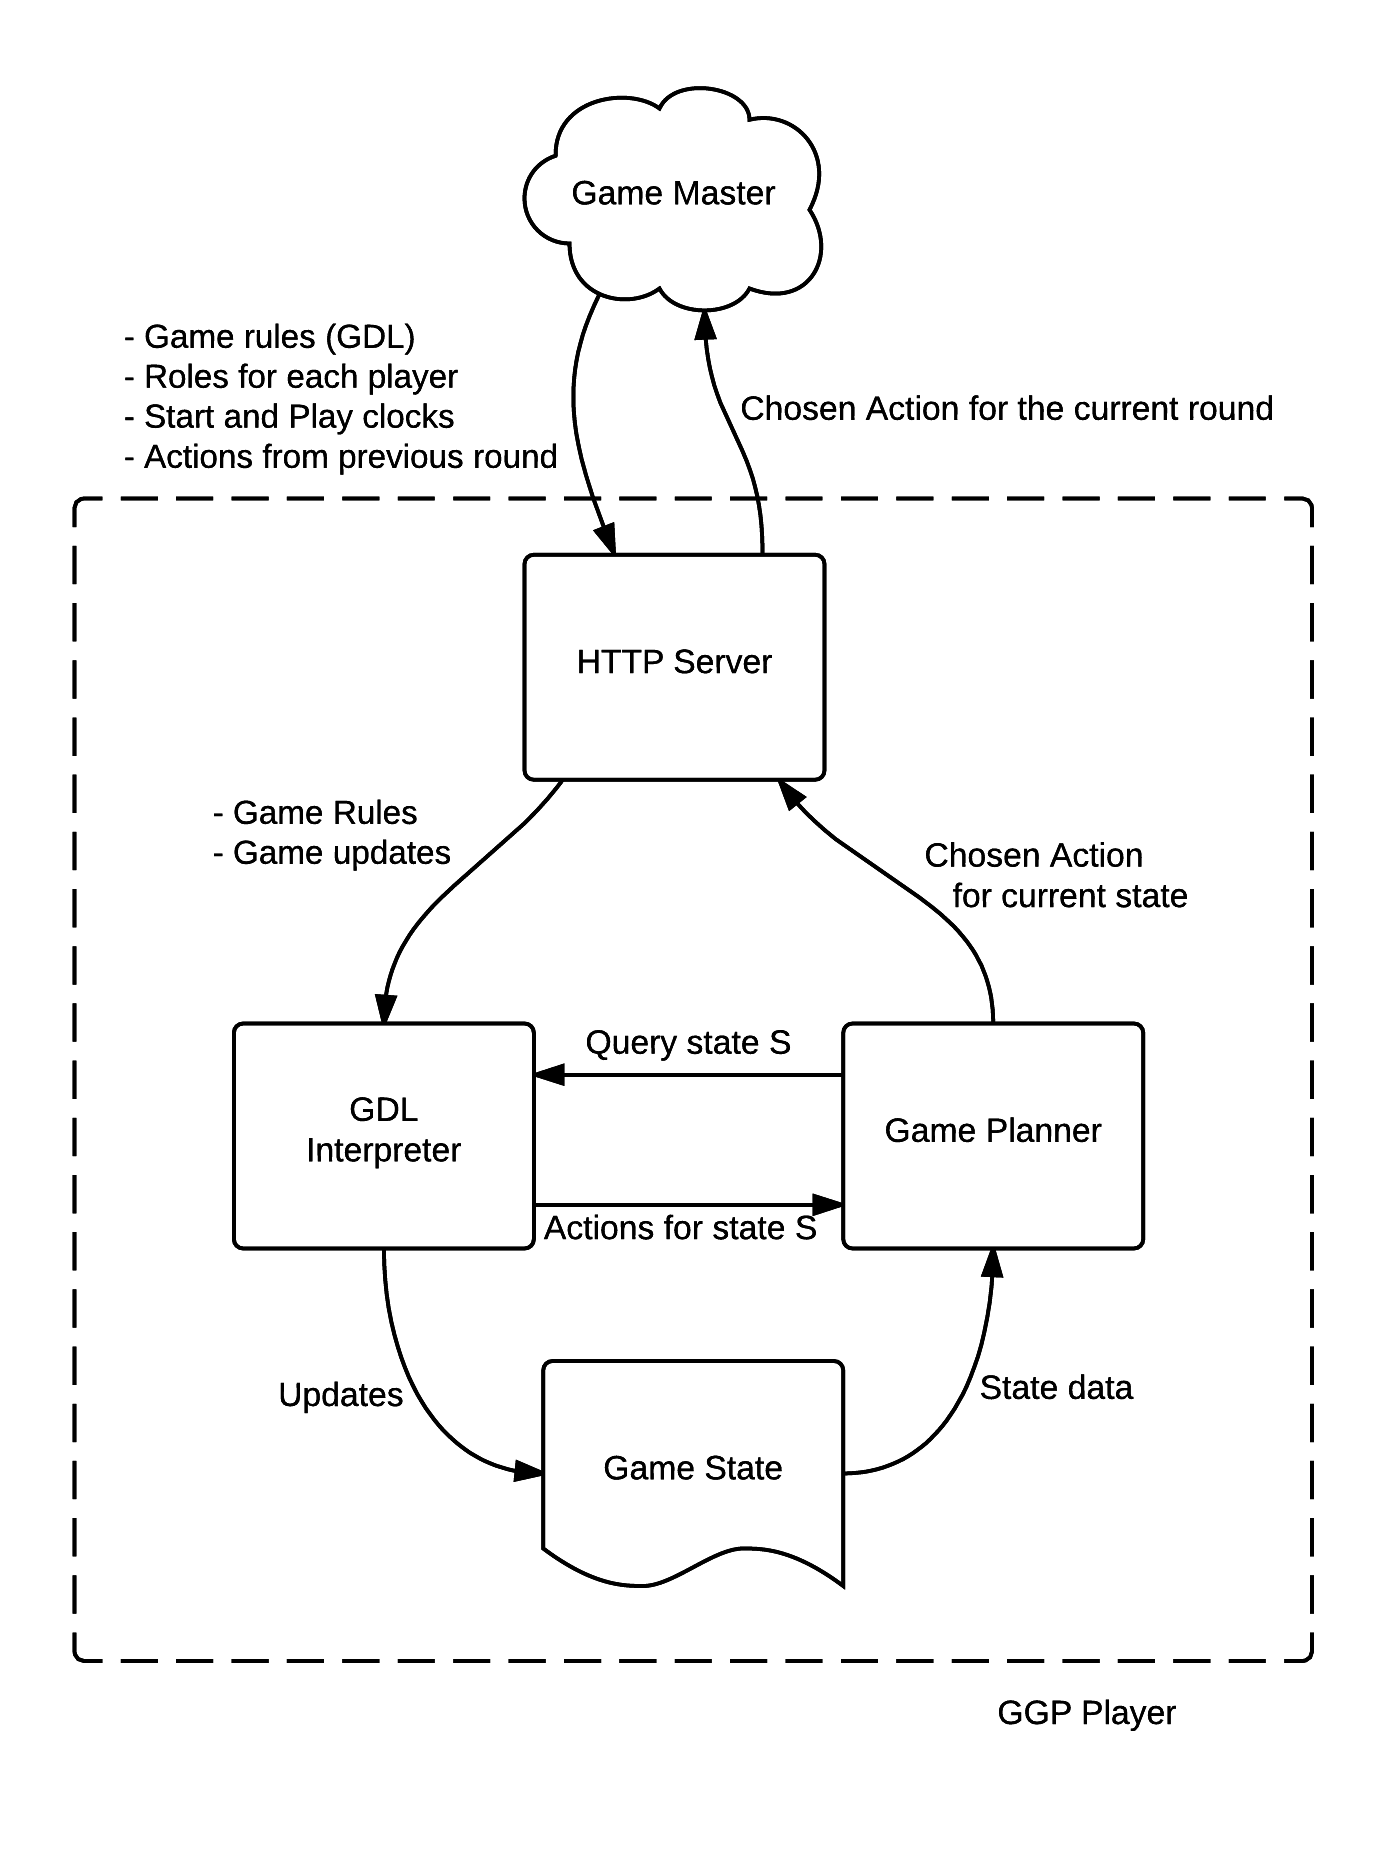
\includegraphics[scale=0.8]{images/GGPplayer.png}
    \caption{Simplified example of a GGP Player architecture}
    \label{fig:player architecture}
\end{figure}

The Game Planner is the biggest factor for system performance, as it is both the component that chooses the strategy and the one that requires the most computing power. The Reasoner can also affect performance in a smaller but relevant way by using a significant portion of the computational power of the system. It becomes more important as more simulations are needed.

The currently most relevant solutions for both Game Planning and GDL interpretation are discussed in chapter \ref{chapter:state_of_the_art}.

\subsection{Measuring performance}
\label{sssec:MeasuringPerformance}

The measurement of game player performance is a hard task in itself. A simple method is playing against a random player (a player that randomly chooses one of the legal actions for each turn). It's no longer very useful because after a certain level of competence can player can beat the random player nearly all the time, so it becomes impossible to distinguish game players based on this metric alone.

What is more commonly done is competition with other existing game players. This should be done in as many different games and types of games as possible, since playing just a few games well is of little value in General Game Playing.

A very useful service is provided by ggp.org, the Tiltyard game server (tiltyard.ggp.org). It constantly arranges matches between the registered players and assigns an Agon skill rating to each player, based on the results. The Agon skill rating is very similar to the EloRank in Chess, except it also takes into account the perceived difficulty of the game and of playing a certain rule in that game.

\subsubsection{Agon Skill}
\label{sssec:AgonSkill}

The Agon rating system computes a skill rating for each player, and a difficulty rating for each role in each game, based on historical match data. This system is based on the Elo rating system for Chess, expanding it in ways that are important for GGP: support for single-player games, many-player games, asymmetric games, cross-game skill ratings, and so on.

For a more detailed understanding of how Agon Skill is calculated, see appendix \ref{appendix:AgonSkill}


\section{Reasoner Techniques}
A \gls{GDL} description by itself isn't sufficient to know what actions are possible at each game state, such features must be deduced from the game rules.
There are two main ways of dealing with this:
Interpreting the rules whenever necessary or converting the game rules to an efficient data structure. The first solution is generally simpler to implement but has sub-par performance. There are, of course, various possible data structures to store the game rules, only one is explored here, \textit{propositional networks}, as it has become very popular in recent works.


\subsection{Propositional networks}

Propositional networks are bidirectional graphs similar to simple logic circuits.
This representation has 2 main benefits: compactness and simplified game analysis.
The compactness comes from the fact that the number of represented states can be exponential to the number of propositions, $n$ propositions can represent $2^{n}$ states, being much more compact than a state machine.

Propositional networks exploit the fact that, in the vast majority of games, there is limited influence to each action: each game symbol is affected only by a few other symbols, not all of them. For example, moving a pawn in Chess only changes the position of the moved pawn and perhaps an opponents piece is taken, the remaining pieces keep their previous state.

The simplified analysis comes from the fact that it becomes simpler to recognize things like symmetries, dead states, composite games (a game composed of multiple games that don't affect each other) and other properties. 

Detecting composite games can be especially important: If a game is, for example, playing 3 board games concurrently and trying to win at least 2 out of the 3, it can lead a player to evaluate all 3 boards when a piece is moved on a single one. However, if the player can detect that the game is composed of 3 smaller games it can factorize it, playing each of the three board games as independent of each other, which is a much more efficient way of handling it.

The components of a basic propositional network can be seen in \ref{fig:propnets components}.

\begin{figure}[h]
	\centering
    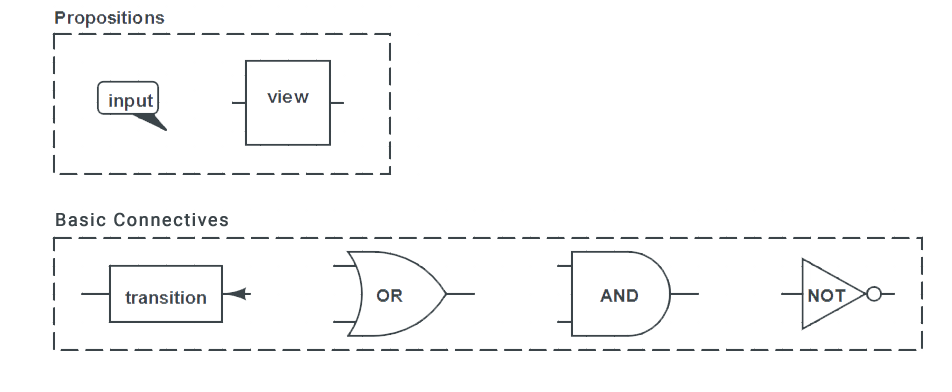
\includegraphics[scale=0.45]{images/propnets_components.png}
    \caption{Basic components of propositional networks}
    \label{fig:propnets components}
\end{figure}

Propositions are boolean valued and can represent things like action legality, if a piece is in a certain location, etc. A proposition is an \textit{input} if it's value is independent of the rest of the network and a \textit{view} if it's the result of a connective.
Connectives are transformations applied to propositions and be a transition or one of the 3 basic logic functions: \textit{and, or} or \textit{not}. A transition acts similarly to a register, its output does not changes until the game moves to the next state. A \textit{view} after a transition is called a \textit{base}.

A simple example of a propositional network can be seen in \ref{fig:propnets example}.

\begin{figure}[h]
	\centering
    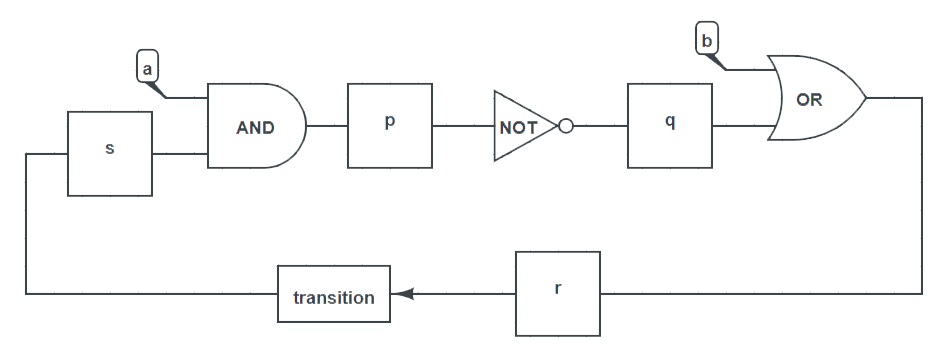
\includegraphics[scale=0.45]{images/propnets_example.png}
    \caption{Example of a propositional network with 2 inputs and 1 transition}
    \label{fig:propnets example}
\end{figure}


\section{Game Planner Techniques}

Some of the most widely used techniques for game planners are summarized bellow. Note that several of the top players actually use more than one technique, for example using an heuristic based approach for single player games, where the player is in charge of all actions.


\subsection{Monte Carlo Tree Search}
Introduced to the GGP competition by CADIA player in 2007, \gls{MCTS} is currently the most used and successful method in GGP. Starting from the current state, the algorithm traverses the tree until the move timer ends, doing as many iterations as possible.

Each iteration has four steps: selection, expansion, simulation and back propagation:

\begin{enumerate}

\item Selection: Some technique is used to select which already traversed node to start from for a search. The most common technique is Upper Confidence Bounds applied for Trees (UCT), described in section \ref{sssec:UCT}.

\item Expansion: Adding a node with the first unvisited state yet to the tree, meaning a state that wasn’t already in the tree.

\item Simulation: Perform a random simulation until a terminal game state is reached.

\item Back-Propagation: The scores obtained by all players at the end of the simulation are back-propagated to all nodes traveled in the selection and expansion stages. This is how the rewards of non-terminal states is computed.

\end{enumerate}

The success of MCTS can be mostly attributed to it not requiring any game-specific knowledge, although this can become a problem if other techniques like heuristics become advanced enough at learning important features of games, as heuristic search can be much faster than simulation. MCTS also has the advantage of parallelizing well. The biggest problems for MCTS are games that can have infinite moves without ending and tree size.

There have been several suggested improvements to the basic MCTS, although most aren’t very thoroughly tested yet. One of the most interesting ones is Simulation Heuristics, proposed by MINI-Player, which aims to add some sort of learning to the standard MCTS algorithm. The heuristics proposed are very light-weight and are the following:

\begin{itemize}

\item Random: The standard MCTS

\item History Heuristic: Tries to identify globally good actions (generally good regardless of state)

\item Mobility: Favors actions that lead to states with more move options relatively to other players.

\item Approximate Goal Evaluation: Tries to calculate the degree of satisfaction of a GDL goal rule.

\item Exploration: Measures the difference between states as a way to do a diverse exploration.

\item Statistical Symbol Counting: Before the start clock simulations are done to calculate the correlation between game score and certain game symbols (moves, pieces, board locations, etc). Symbols that do not change much are then ignored to allow more computation to be made on the more relevant ones.

\end{itemize}

\subsubsection{UCT}
\label{sssec:UCT}

Upper Confidence Bounds applied for Trees (UCT) is a way of selecting what node should be searched next and it's widely used for the \textit{Selection} stage of \gls{MCTS}. It uses a constant that can be tweaked to favor more or less exploration of non visited branches. The UCT algorithm is described by \ref{UCT}:

\begin{center}
\begin{equation} \label{UCT}
a^{*} = arg \max_{a\in A(s)} \left \{ Q(s,a) + C \sqrt{\frac{\ln|N(s)|} {N(s,a)}} \right \}
\end{equation}
\end{center}

Where $a^{*}$ is the selected node, $a \in A(s)$ means an action that contained in the set of possible actions in the current state $s$, $Q(s,a)$ is an assessment of performing $a$ in state $s$, $C$ is the exploration ratio constant, $N(s)$ is the number of previous visits to state $s$ and $N(s,a)$ is the number of times $a$ has been sampled in state $s$.

\subsubsection{RAVE}

\subsection{Heuristic based techniques}
Heuristics are methods that simplify or accelerate problem solving by not guaranteeing optimal solutions but satisfying approximations. Heuristics can be very useful whenever finding an optimal solution is impossible or impractical.

In the case of \gls{GGP} these techniques try to learn or identify features of the game, so the player can more efficiently approximate the quality of the available actions. For example, a simple heuristic for Checkers would be to count the difference in pieces between the two players. One of the biggest drawbacks of this type of technique is that heuristics become less useful the more general they become, meaning that, ideally, specialized heuristics should be created at run time, which is a very complex problem.

By using heuristics to attach a value to game states and/or actions, it is then possible to use search algorithms to try to find the best strategy.
It's important to note that the performance of these search algorithms is completely dependent on the quality of the heuristics on top of which they run.

These techniques can be used in a game player by themselves but they can also be used to improve \gls{MCTS} based players.

\subsubsection{MinMax}

MiniMax is a depth-first heuristic search method for adversary games.
It is centered around the simple assumption that opponents try to minimize our score while we try to maximize it. 

A MinMax game tree is represented in figure \ref{fig:min_max}, where \textit{square} plays against \textit{circle}. The value in each node is the value of the state for \textit{square} (based on the chosen heuristic). Squares represent states where \textit{square} has control, similarly for circles.

Running the MinMax algorithm for \textit{square}, we'll start with a depth-fisrt traversal of the tree, first finding the leaves on the left side, with values 5 and 6. Since in the previous turn the opponent (\textit{circle}) is in control, 5 will be the chosen state if the game is ever in the parent state, since \textit{circle} is trying to minimize \textit{square}'s value. 
The value 5 is then propagated to the parent of both leaves, and the same method is applied to all other leaves and direct parents. We now do a similar process for all the nodes in the 4th level, as an example we can use the leftmost nodes, 5 and 4: Since these nodes represent \textit{circle}'s turn, that means in the previous turn \textit{square} is in control, and will try to maximize his value, choosing the action that leads to a state with value 5. After following these maximizing and minimizing rules, we end up with the maximum attainable value at the root (current state) node.

This algorithm can be easily generalized to games with more than one opponent, by assuming all opponents are working together against us and representing them as a single opponent that takes multiple consecutive turns. This is very pessimistic model of the opponents, since they are probably competing among themselves as well. The performance of the algorithm will of course depend on how the deep the search can go, on how close the opponent behaves to this model and the heuristics correlation between the heuristics used and game results.


\begin{figure}[h]
	\centering
    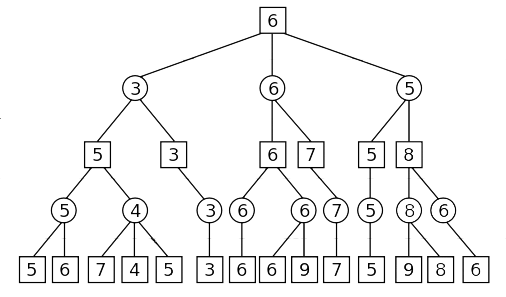
\includegraphics[scale=0.8]{images/min_max.png}
    \caption{Example of a MinMax game tree}
    \label{fig:min_max}
\end{figure}

\subsubsection{Alpha-Beta Pruning}

MinMax can be very expensive as it tries to search through the whole game tree. Alpha-Beta Pruning is a very effective enhancement to MinMax, that attempts to reduce the amount of nodes that need to be visited. 

It works by identifying nodes that lead to sub-trees that cannot change the current game value.
An example can be seen in figure \ref{fig:alpha_beta}: Looking at the right side of the tree we can see that the opponent can choose a state with value 5, meaning whatever values are found in the other children of that state, the value attainable by \textit{square} will not be higher than 5. Since \textit{square} can already get a value of 6 by going for the middle choice, there's no point in searching the other children of the rightmost node because that choice cannot lead to a better score than 5.
This allows for the pruning of many irrelevant sub-trees by simply storing a lower-bound, $\alpha$, and an upper-bound, $\beta$, for each level of the tree.

\begin{figure}[h]
	\centering
    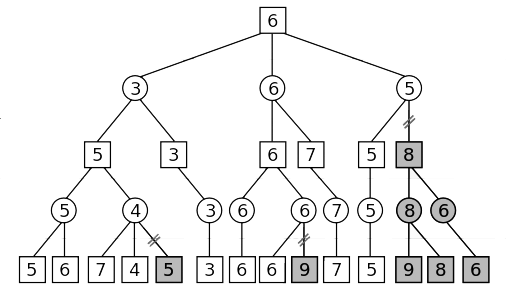
\includegraphics[scale=0.8]{images/alpha_beta.png}
    \caption{Example of a pruned game tree}
    \label{fig:alpha_beta}
\end{figure}


%\subsubsection{FluxPlayer}
%The winner of the second GGP competition, in 2006, this player used fuzzy logic to determine how close to terminal a certain state is.
%
%Fuzzy logic is a form of logic that allows multiple different values beyond True or False, and also allows overlap between these values. For example: water can be considered cold, warm or hot, but also warm and hot at the same time, since for some temperatures it is not clear which one is the correct one. Fuzzy logic also allows each of these states to have varying degrees of certainty: the water can be 80\% warm and 10\% cold, allowing conditions like if water is very warm: add some cold water, where the very keyword is also part of the fuzzy logic implementation.
%
%The system also used a novel heuristic search that could be computed from the specifications of the game.